\begin{figure*}[t]
    \centering
    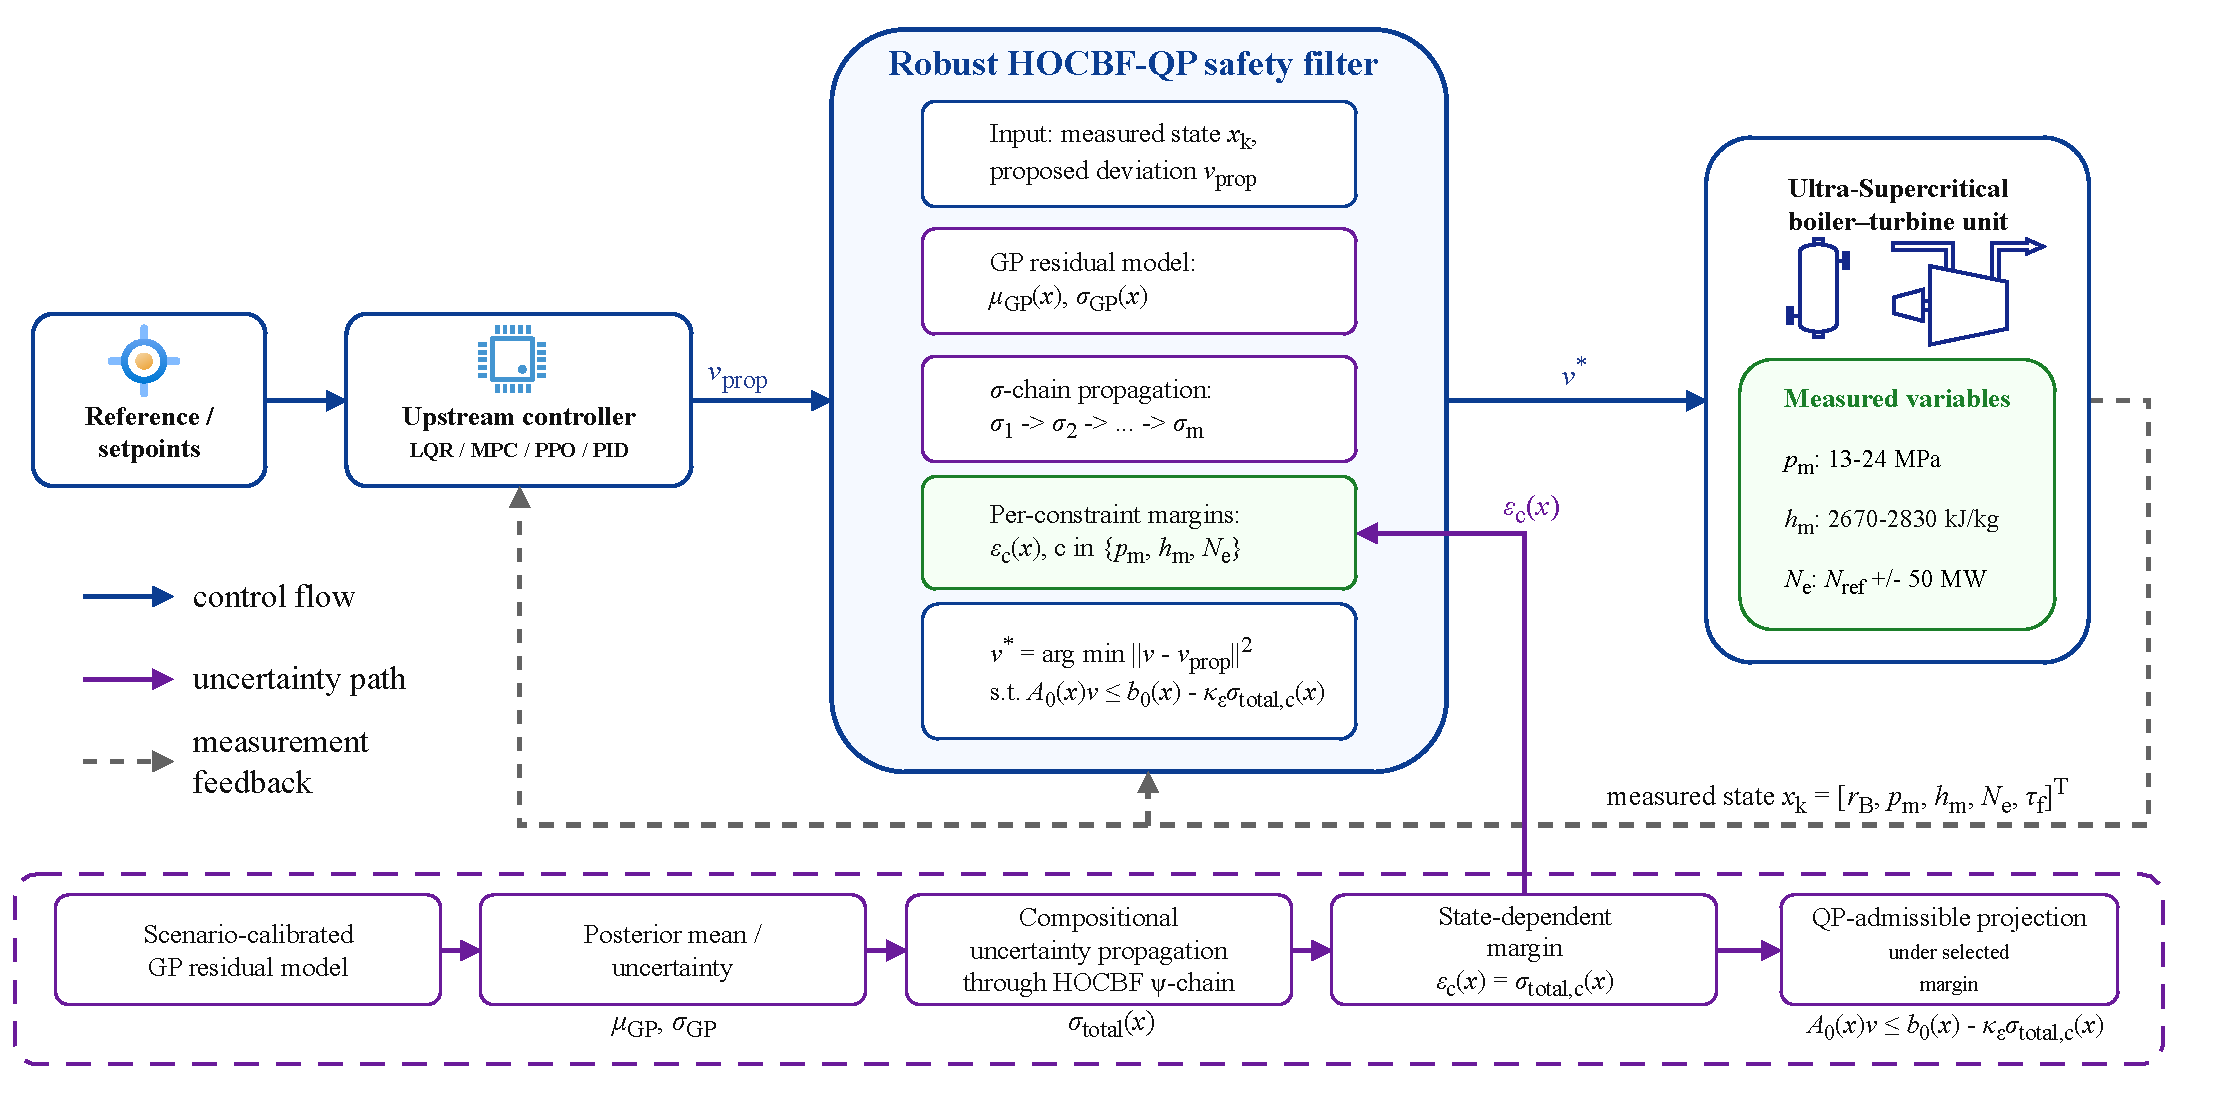
\includegraphics[width=0.92\textwidth]{figures/Figure_1.pdf}
    \caption{Process-control-oriented architecture of the Robust HOCBF safety filter. An upstream controller (LQR, MPC, PPO, or classical) proposes an action $u_{\mathrm{prop}}$; the Robust HOCBF-QP projects it to the nearest safe action $u^*$ satisfying $A_0 u \le b_0 - \epsilon(x)$. A GP residual model learns the drift mismatch $\Delta f$ from process data and supplies mean correction $\mu_{\mathrm{GP}}$ and per-dimension posterior variance $\sigma_{\mathrm{GP}}$ to the compositional $\sigma$-chain, which computes the per-constraint, relative-degree-aware robustness margin $\epsilon(x)$.}
    \label{fig:architecture}
\end{figure*}
